\section{Evaluation}
\subsection{Storage systems latency.}
\par First we use Flexible I/O (FIO) Tester and create micro benchmarks to understand how much latency each different storage system adds. We configure FIO to use the libaio engine, random reads, direct I/O, 512 bytes and 4KB block size, 1 I/O depth and 1 thread.
\par Figure \ref{fig:fio_512} shows the FIO report of latency with 512 request size of each storage system. "r" stands for ramdisk and "n" stands for NVMe, "OF" stands for NVMe-oF with SPDK User-Space drivers.
\begin{figure}[H]
  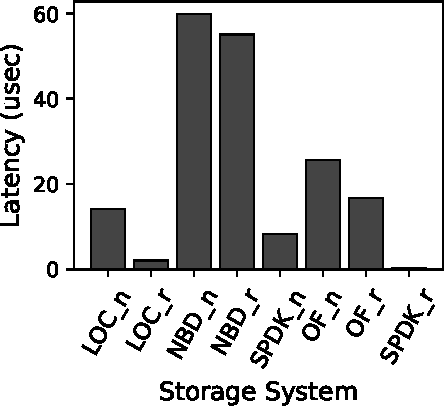
\includegraphics[width=\linewidth]{asplos25-Thesis/figures/fio_512.pdf}\\
\caption{Average latency (usec) of local and remote storage systems with 512B request size.}
\label{fig:fio_512}
\end{figure}
Local NVMe haves an average of 14.16 usec latency and local ramdisk 2.04 usec 6.94× better. Exported NVMe with NBD (TCP) latency is 4.22× higher than local with an average of 59.86 usec. By looking at the Exported ramdisk with NBD (TCP) average latency we can see that it is very close to NBD NVMe with 55.11 usec only 1.08× better now, meaning that there is a common overhead. This overhead can either be the NBD I/O path or high TCP latency. We use Netperf to measure the TCP latency and conduct experiments with 512 bytes of data in each packet. Netperf reports 37.84 usec average latency. Adding local NVMe and TCP latency we have 52 usec very close to the NBD (TCP) latency 59.86 usec. We conclude that the overhead here is TCP which takes 63.2\% of the average latency of NBD NVMe. 
\par Moving on we try to lower the latency of the local I/O path to the device by using userspace drivers (SPDK). We run FIO to the NVMe with SPDK User-Space drivers and we get 8.31 usec average latency 1.7 × better. We also try to lower the network latency with NVMe-oF NVMe with SPDK User-Space drivers and we measure 25.69 usec average latency. Here SPDK ramdisk outperforms everything with 0.33 usec average latency, but the NVMe-oF ramdisk with SPDK User-Space drivers haves 16.66 usec average latency closer to the NVMe-oF NVMe only 1.54× better compared to the local performance where the local ramdisk is 25.18× better. We can also say here that there is a common overhead. This overhead can either be the NVMe I/O path or high Network latency. Previously we measured the NVMe with SPDK User-Space drivers and we got 8.31 usec a logical 32.34\% of the NVMe-oF NVMe with SPDK latency. We used ib\_read\_lat to conduct RDMA Read Latency Test with 512 bytes requests and we measure that the infiniband ports average latency is 2 usec only 7.78\% of the NVMe-oF NVMe with SPDK latency meaning that the high latency can be by the Linux Kernel NVMe-oF Initiator. Unfortunately, SPDK's user-space NVMe-oF initiator doesn't directly create block devices in /dev, SPDK uses its own bdev (block device) layer which will not be compatible for later experiments with TeraHeap. 
\par The NVMe-oF NVMe with SPDK achieving 25.69 microseconds and the NVMe-oF ramdisk with SPDK reaching 16.66 microseconds average latency (nearly as fast as the local NVMe at 14.16 microseconds) are suitable to proceed with our evaluation using Teraheap.
\par Similarly with 4KB block size we get the same overheads as shown in figure \ref{fig:fio_4k}. Here FIO reports more latency for moving the 4KB data locally and/or across network.

\begin{figure}[H]
  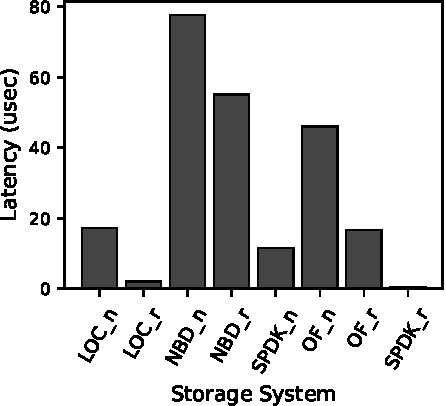
\includegraphics[width=\linewidth]{asplos25-Thesis/figures/fio_4k.pdf}\\
\caption{Average latency (usec) of local and remote storage systems with 4KB request size.}
\label{fig:fio_4k}
\end{figure}

\subsection{TeraHeap performance with NVMe-oF}
\par This section compares TeraHeap performance of two set ups one with local NVMe device and one with NVMe-oF exported NVMe with SPDK User-Space drivers. Figure \ref{fig:bench_spark} illustrates the performance of TeraHeap with Spark workloads for both setups.
\begin{figure}[H]
  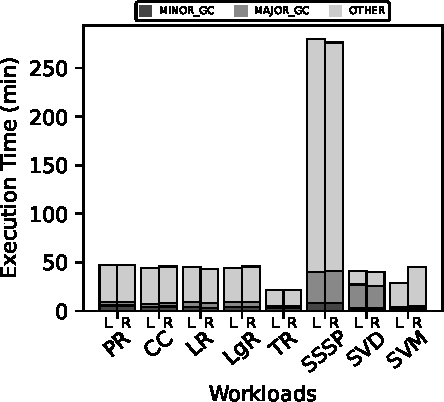
\includegraphics[width=\linewidth]{asplos25-Thesis/figures/bench_spark.pdf}\\
\caption{TeraHeap Spark performance. local NVMe device (L) compared to NVMe-oF exported NVMe with SPDK (R).}
\label{fig:bench_spark}
\end{figure}
The two setups local NVMe device (L) and NVMe-oF exported NVMe with SPDK (R) with TeraHeap perform similarly with Spark workloads. Spark Workloads read objects from H2 but they don't change them, with spark heavy Write operations are missing. We can see that local setup outperforms the remote setup in Pagerank(PR), Connected Components(CC) and Logistic Regression(LgR) making the local setup 0.85\%, 3.55\% and 3.18\% faster accordingly. The big difference is in the SVM workload where the local setup outperforms the remote by 37.30\% \textbf{(why????)}. There are also cases where the remote setup is better. Workloads Linear Regression(LR), Triangle Counts(TR), Shortest Path(SSSP) and SVDPlusPlus(SVD) report that the remote setup is 4.76\%, 2.08\%, 1.37\% and 2.76\% quicker accordingly.
\par Next we run Teraheap with the Giraph Workloads. These workloads read objects from H2 and also can change them. Here we expect heavy write operations that can stress the remote setup. Figure \ref{fig:bench_giraph} illustrates the performance of TeraHeap with Giraph workloads for both setups NVMe device (L) and NVMe-oF exported NVMe with SPDK (R).
\begin{figure}[H]
  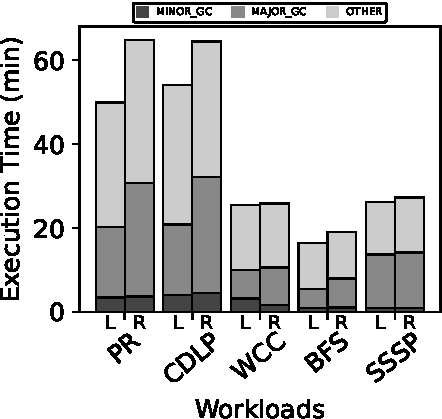
\includegraphics[width=\linewidth]{asplos25-Thesis/figures/bench_giraph.pdf}\\
\caption{TeraHeap Giraph performance. local NVMe device (L) compared to NVMe-oF exported NVMe with SPDK (R).}
\label{fig:bench_giraph}
\end{figure}
Here, due to the write operations, the remote setup (R) never manages to exceed the performance of the local setup (L). PageRank (PR), CDLP and BFS workloads are the ones that the remote setup struggles the most with local setup being 22.97\% 16.24\% and 13.07\% quicker accordingly. In the setups mentioned before the remote setup is losing performance due to major GC's taking more time to complete. Following up with WCC and SSSP workloads we can see that the local setup is only 1.54\%	and 3.97\% faster again here major GC's are the reason the remote setup is slower.

\subsection{Workload disk statistics}

\par In this section we review the disk statistics of the workload runs. First we examine Spark figures \ref{fig:spark_r} and \ref{fig:spark_w} show reads and writes accordingly. First we can confirm that reads are more than writes due to the nature of spark benchmarks. Next focusing on the reads we can see that the Gigabytes read for both the local setup (L) and the remote setup (R) are close. An exception here is the SVM workload where the remote setup haves 8.3× more Gigabytes of reads.
\par Next we examine Giraph figures \ref{fig:giraph_r} and \ref{fig:giraph_w} show reads and writes accordingly. We can confirm that writes are close or more than reads due to Giraph benchmarks changing off-heap objects. focusing on the writes we can see that the Gigabytes wrote for both the local setup (L) and the remote setup (R) are close. In the PageRank(PR)	and CDLP workloads where the local setup (L) outperforms the most of the remote setup (R) (figure \ref{fig:bench_giraph} 22.97\% and 16.24\% faster) we can see more reads (figure \ref{fig:giraph_r}) for the remote setup due to more major GC's.

\begin{figure}[H]
  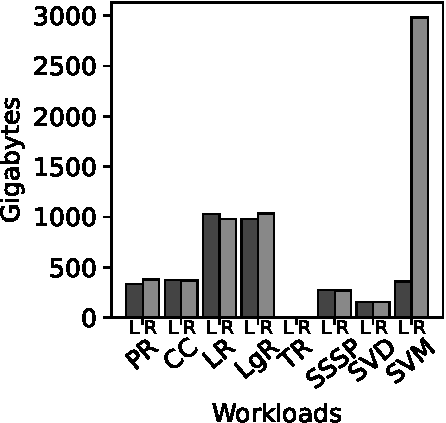
\includegraphics[width=\linewidth]{asplos25-Thesis/figures/spark_r.pdf}\\
\caption{Teraheap Spark workloads reads (GB). local NVMe device (L) compared to NVMe-oF exported NVMe with SPDK (R).}
\label{fig:spark_r}
\end{figure}
\begin{figure}[H]
  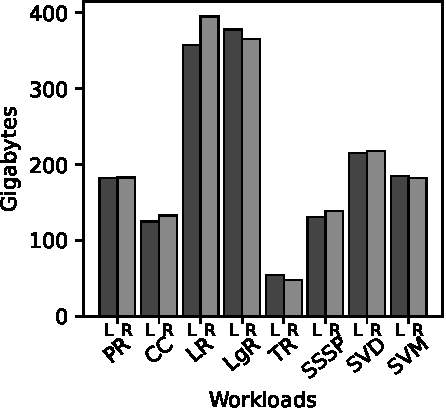
\includegraphics[width=\linewidth]{asplos25-Thesis/figures/spark_w.pdf}\\
\caption{Teraheap Spark workloads writes (GB). local NVMe device (L) compared to NVMe-oF exported NVMe with SPDK (R).}
\label{fig:spark_w}
\end{figure}
\vspace{10em}
\begin{figure}[H]
  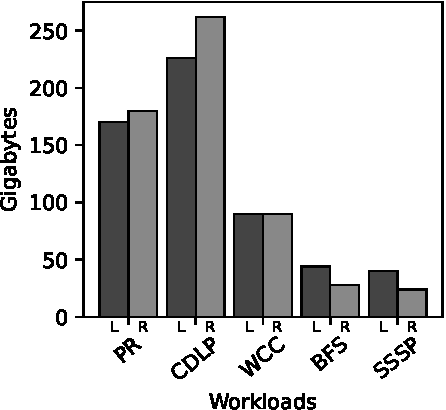
\includegraphics[width=\linewidth]{asplos25-Thesis/figures/giraph_r.pdf}\\
\caption{Teraheap Giraph workloads reads (GB). local NVMe device (L) compared to NVMe-oF exported NVMe with SPDK (R).}
\label{fig:giraph_r}
\end{figure}

\begin{figure}[H]
  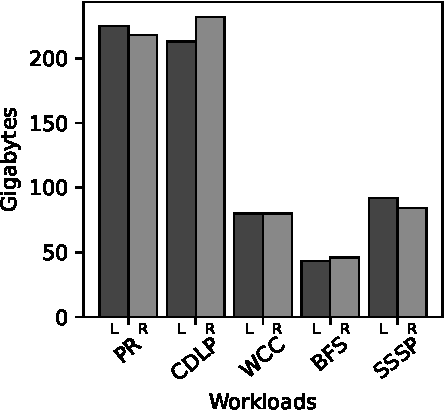
\includegraphics[width=\linewidth]{asplos25-Thesis/figures/giraph_w.pdf}\\
\caption{Teraheap Giraph workloads writes (GB). local NVMe device (L) compared to NVMe-oF exported NVMe with SPDK (R).}
\label{fig:spark_w}
\end{figure}
%\begin{itemize}
 %   \item start by explaining FIO results and that we will focus on latency
  %  \item show fio results explain the graph (break down loc numbers, say nbd is slow-show netperf tcp latency number, break down spdk numbers(reference to sequential FIO latency number-cache hit))
  %  \item show infiniband numbers (add an ib-read-lat subsection in methodology)
   % \item show spark , giraffe numbers comment on faster or slower times with percentages
    %\item show disk stats numbers and plots to back down heavy I/O workloads
%\end{itemize}